\documentclass[12pt,a4paper]{article}
\usepackage[utf8]{inputenc}
\usepackage[margin=1in]{geometry}
\usepackage{graphicx}
\usepackage{amsmath}
\usepackage{amsfonts}
\usepackage{amssymb}
\usepackage{enumitem}
\usepackage{fancyhdr}
\usepackage{titlesec}
\usepackage{tikz}
\usepackage[normalem]{ulem}

\usetikzlibrary{shapes,positioning,calc}
% Page setup
\pagestyle{fancy}
\fancyhf{}
\rhead{CSE 414 - Assignment 03}
\lhead{Database Design Using E-R Model}
\cfoot{\thepage}

% Title formatting
\titleformat{\section}{\Large\bfseries}{\thesection}{1em}{}
\titleformat{\subsection}{\large\bfseries}{\thesubsection}{1em}{}

\begin{document}

% Title Page
\begin{titlepage}
    \begin{figure}[htbp]
    \centering
    \includegraphics[width=0.2\textwidth]{cu.png}
    \end{figure}
    \centering
    \vspace*{0.5cm}
    {\Huge\bfseries University of Chittagong}\\[0.5cm]
    {\Large Department of Computer Science \& Engineering}\\[0.5cm]
    {\large Database Systems Lab}\\[2cm]
    
    {\large Name of the assignment:}\\[0.3cm]
    {\LARGE\bfseries Database Design using E-R Model}\\[0.5cm]
    {\large CSE 414}\\[0.5cm]
    {\large Assignment 03}\\[3cm]
    
    \begin{minipage}[t]{0.4\textwidth}
    \raggedleft
    Submitted By:\\
    \large \textbf{Debashish Chakraborty}\\
    \large ID: 23701034
    \end{minipage}
    \hspace{0.05\textwidth}
    \vrule width 1pt
    \hspace{0.05\textwidth}
    \begin{minipage}[t]{0.4\textwidth}
    Submitted To:\\
    \large \textbf{Dr. Rudra Pratap Deb Nath}\\
    \large Associate Professor
    \end{minipage}
    
    \vfill
    {\large June 10, 2025}
\end{titlepage}

\newpage


\section*{Problem 6.1}

\textbf{Problem:} Construct an E-R diagram for a car insurance company whose customers own one or more cars each. Each car has associated with it zero to any number of recorded accidents. Each insurance policy covers one or more cars and has one or more premium payments associated with it. Each payment is for a particular period of time, and has an associated due date, and the date when the payment was received.
\\
\textbf{Solution:}

\begin{center}
% Space for ER diagram image
\includegraphics[width=1\textwidth]{6.1.png}
\end{center}

The E-R diagram includes entities: customer, car, accident, policy, and payment with appropriate relationships and attributes as shown above.

\section*{Problem 6.2}
\subsection*{6.2.a}

Consider a database that includes the entity sets student, course, and section from the university schema and that additionally records the marks that students receive in different exams of different sections.
\\ \\
\textbf{Problem:} Construct an E-R diagram that models exams as entities and uses a ternary relationship as part of the design.
\newpage
\textbf{Solution:}

\begin{center}
% Space for ER diagram image
\includegraphics[width=0.9\textwidth]{6.2.a.png}
\end{center}

\subsection*{6.2.b}

\textbf{Problem:} Construct an alternative E-R diagram that uses only a binary relationship between student and section. Make sure that only one relationship exists between a particular student and section pair, yet you can represent the marks that a student gets in different exams.

\textbf{Solution:}

\begin{center}
% Space for ER diagram image
\includegraphics[width=1\textwidth]{6.2.b.png}
\end{center}

\section*{Problem 6.3}

\textbf{Problem:} Design an E-R diagram for keeping track of the scoring statistics of your favorite sports team. You should store the matches played, the scores in each match, the players in each match, and individual player scoring statistics for each match. Summary statistics should be modeled as derived attributes with an explanation as to how they are computed.
\\
\textbf{Solution:}

\begin{center}
% Space for ER diagram image
\includegraphics[width=1\textwidth]{6.3.png}
\end{center}

The diagram includes match and player entities with a score relationship. The season\_score attribute for players is a derived attribute computed by summing all individual match scores for that player.

\section*{Problem 6.5}

\textbf{Problem:} An E-R diagram can be viewed as a graph. What do the following mean in terms of the structure of an enterprise schema?

\subsection*{The graph is disconnected}

\textbf{Solution:}  A disconnected graph implies that there are pairs of entity sets that are unrelated to each other. In an enterprise schema, we can say that the two parts of the enterprise are completely independent of each other. If we split the graph into connected components, we have a separate database corresponding to each independent part of the enterprise.

\subsection*{The graph has a cycle}

\textbf{Solution:} A path in the graph between a pair of entity sets indicates a relationship between the two entity sets. If there is a cycle in the graph, then every pair of entity sets on the cycle are related to each other in at least two distinct ways. If the E-R diagram is acyclic, then there is a unique relationship between every pair of entity sets.

\section*{Problem 6.7}

\textbf{Problem:} A weak entity set can always be made into a strong entity set by adding to its attributes the primary-key attributes of its identifying entity set. Outline what sort of redundancy will result if we do so.

\textbf{Solution:} When a weak entity set is made into a strong entity set by adding the primary key attributes of its identifying entity set, the resulting redundancy comes from repeating the identifying entity’s key attributes in every tuple of the formerly weak entity set, which can cause several types of data redundancy and anomalies. Such as: 
\begin{itemize}
\item 
\textbf{Repetition of Primary Key Attributes:} Every tuple in the (now strong) entity set must include the full primary key of the identifying entity.

If the identifying entity has a long composite key, this leads to a lot of repeated data.

\item \textbf{Data Duplication:}

Any shared identifying entity attribute (like a name, date, etc.) would be duplicated in each weak entity tuple.
\end{itemize}
\section*{Problem 6.9}

\textbf{Problem:} Suppose the advisor relationship set were one-to-one. What extra constraints are required on the relation advisor to ensure that the one-to-one cardinality constraint is enforced?

\textbf{Solution:} To enforce a one-to-one relationship in the advisor table, we declare both $Student_{ID}$ and $Instructor_{ID}$ as superkey.

Add \textbf{UNIQUE} constraints on both $Student_{ID}$ and $Instructor_{ID}$.

This guarantees that no student or instructor appears more than once in the relation, satisfying the one-to-one cardinality.

\section*{Problem 6.13}

\textbf{Problem:} An E-R diagram usually models the state of an enterprise at a point in time. Suppose we wish to track temporal changes, that is, changes to data over time. For example, Zhang may have been a student between September 2015 and May 2019, while Shankar may have had instructor Einstein as advisor from May 2018 to December 2018, and again from June 2019 to January 2020. Similarly, attribute values of an entity or relationship, such as title and credits of course, salary, or even name of instructor, and tot\_cred of student, can change over time.

One way to model temporal changes is as follows: We define a new data type called valid\_time, which is a time interval, or a set of time intervals. We then associate a valid\_time attribute with each entity and relationship, recording the time periods during which the entity or relationship is valid. The end time of an interval can be infinity; for example, if Shankar became a student in September 2018, and is still a student, we can represent the end time of the valid\_time interval as infinity for the Shankar entity. Similarly, we model attributes that can change over time as a set of values, each with its own valid\_time.

\subsection*{6.13.a}Draw an E-R diagram with the student and instructor entities, and the advisor relationship, with the above extensions to track temporal changes.\\

\textbf{Solution:}

\begin{figure}[h]
\centering
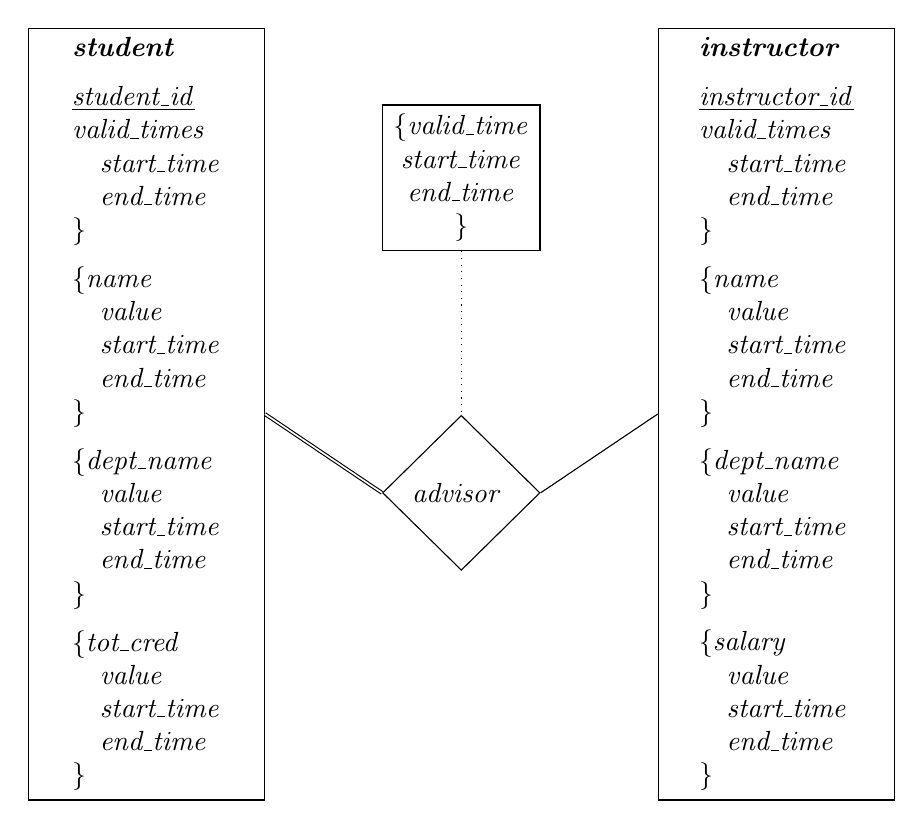
\begin{tikzpicture}[
    entity/.style={rectangle, draw, minimum width=3cm, minimum height=8cm, align=left},
    relationship/.style={diamond, draw, minimum width=2cm, minimum height=1.5cm, align=center},
    attribute/.style={rectangle, draw, minimum width=2cm, minimum height=1.5cm, align=center},
    node distance=1cm
]

% Student Entity
\node[entity] (student) at (0,0) {
    \textbf{\textit{student}} \\[0.2cm]
    \underline{\textit{student\_id}} \\
    {\textit{valid\_times}} \\
    \quad \textit{start\_time} \\
    \quad \textit{end\_time} \\
    \} \\[0.2cm]
    \{\textit{name} \\
    \quad \textit{value} \\
    \quad \textit{start\_time} \\
    \quad \textit{end\_time} \\
    \} \\[0.2cm]
    \{\textit{dept\_name} \\
    \quad \textit{value} \\
    \quad \textit{start\_time} \\
    \quad \textit{end\_time} \\
    \} \\[0.2cm]
    \{\textit{tot\_cred} \\
    \quad \textit{value} \\
    \quad \textit{start\_time} \\
    \quad \textit{end\_time} \\
    \}
};

% Instructor Entity
\node[entity] (instructor) at (8,0) {
    \textbf{\textit{instructor}} \\[0.2cm]
    \underline{\textit{instructor\_id}} \\
    \textit{valid\_times} \\
    \quad \textit{start\_time} \\
    \quad \textit{end\_time} \\
    \} \\[0.2cm]
    \{\textit{name} \\
    \quad \textit{value} \\
    \quad \textit{start\_time} \\
    \quad \textit{end\_time} \\
    \} \\[0.2cm]
    \{\textit{dept\_name} \\
    \quad \textit{value} \\
    \quad \textit{start\_time} \\
    \quad \textit{end\_time} \\
    \} \\[0.2cm]
    \{\textit{salary} \\
    \quad \textit{value} \\
    \quad \textit{start\_time} \\
    \quad \textit{end\_time} \\
    \}
};

% Valid_time attribute
\node[attribute] (validtime) at (4,3) {
    \{\textit{valid\_time} \\
    \textit{start\_time} \\
    \textit{end\_time} \\
    \}
};

% Advisor relationship
\node[relationship] (advisor) at (4,-1) {
    \textit{advisor}
};

% Lines connecting entities to relationship
\draw[style=double] (student.east) -- (advisor.west);
\draw (instructor.west) -- (advisor.east);

% Dotted line from valid_time to advisor
\draw[dotted] (validtime.south) -- (advisor.north);

\end{tikzpicture}

\caption{E-R diagram for Exercise 6.13.a}
\label{fig:temporal_er}
\end{figure}

\subsection*{6.13.b}Convert the E-R diagram discussed above into a set of relations. \\
It should be clear that the set of relations generated is rather complex, leading to difficulties in tasks such as writing queries in SQL. An alternative approach, which is used more widely, is to ignore temporal changes when designing the E-R model (in particular, temporal changes to attribute values), and to modify the relations generated from the E-R Model to track temporal changes.
\newpage
\textbf{\underline{Solution:}}

\textbf{Student Entity Relations:}
\begin{align}
&\textit{student}(\underline{\textit{student\_id}}) \\
&\textit{student\_valid\_times}(\underline{\textit{student\_id}}, \underline{\textit{start\_time}}, \underline{\textit{end\_time}}) \\
&\textit{student\_name}(\underline{\textit{student\_id}}, \underline{\textit{value}}, \underline{\textit{start\_time}}, \underline{\textit{end\_time}}) \\
&\textit{student\_dept\_name}(\underline{\textit{student\_id}}, \underline{\textit{value}}, \underline{\textit{start\_time}}, \underline{\textit{end\_time}}) \\
&\textit{student\_tot\_cred}(\underline{\textit{student\_id}}, \underline{\textit{value}}, \underline{\textit{start\_time}}, \underline{\textit{end\_time}})
\end{align}

\textbf{Instructor Entity Relations:}
\begin{align}
&\textit{instructor}(\underline{\textit{instructor\_id}}) \\
&\textit{instructor\_valid\_times}(\underline{\textit{instructor\_id}}, \underline{\textit{start\_time}}, \underline{\textit{end\_time}}) \\
&\textit{instructor\_name}(\underline{\textit{instructor\_id}}, \underline{\textit{value}}, \underline{\textit{start\_time}}, \underline{\textit{end\_time}}) \\
&\textit{instructor\_dept\_name}(\underline{\textit{instructor\_id}}, \underline{\textit{value}}, \underline{\textit{start\_time}}, \underline{\textit{end\_time}}) \\
&\textit{instructor\_salary}(\underline{\textit{instructor\_id}}, \underline{\textit{value}}, \underline{\textit{start\_time}}, \underline{\textit{end\_time}})
\end{align}

\textbf{Advisor Relationship Relation:}
\begin{align}
&\textit{advisor}(\underline{\textit{student\_id}}, \underline{\textit{instructor\_id}}, \underline{\textit{start\_time}}, \underline{\textit{end\_time}})
\end{align}



\section*{Problem 6.14}

\textbf{Problem:} Explain the distinctions among the terms primary key, candidate key, and superkey.

\textbf{Solution:}
\begin{itemize}
\item A superkey is any set of attributes that can uniquely identify a tuple (row) in a relation. A superkey may contain extra attributes not necessary for uniqueness.
\item A candidate key is a minimal superkey for which no proper subset is a superkey.Removing any attribute from it would make it no longer uniquely identify tuples.
\item A primary key is the chosen candidate key used as the main identifier for tuples in a table.
\end{itemize}
\newpage
\section*{Problem 6.15}

\textbf{Problem:} Construct an E-R diagram for a hospital with a set of patients and a set of medical doctors. Associate with each patient a log of the various tests and examinations conducted.

\textbf{Solution:}

\begin{center}
% Space for ER diagram image
\includegraphics[width=1\textwidth]{6.15.png}
\end{center}

The diagram shows Patient, Medical Doctor, and Tests and Examinations entities. patientTests is a ternary relationship set.

And also we make the testsAndExaminations entity a weak entity having identifying entity set Patient. And then adding a relationship set between the weak entity testsAndExaminations and MedicalDoctor, representing which medical doctor performed which test and examination. In fact doing that has the added benefit of constraining each entity in testsAndExaminations to a single Patient.

But using a ternary relationship as depicted in the above diagram also has its benefits. For example, if a group of patients are tested and examined by the same type of test and have the same result, we might associate each of the patients in the group to the same entity in testsAndExaminations.

\section*{Problem 6.19}

\textbf{Problem:} We can convert any weak entity set to a strong entity set by simply adding appropriate attributes. Why, then do we have weak entity sets?\\
\\
\textbf{Solution:} We have weak entity sets because we want to make the dependence of the weak entity set on its identifying/owning entity set explicit.

\section*{Problem 6.21}
\begin{center}
% Space for ER diagram image
\includegraphics[width=0.6\textwidth]{6.21Question.png}
\end{center}
 Consider the E-R diagram in Figure 6.30, which models an online bookstore.

\subsection*{6.21.a} Suppose the bookstore adds Blu-ray discs and downloadable video to its collection. The same item may be present in one or both formats, with differing prices. Draw the part of the E-R diagram that models this addition, show just the parts related to video.\\

\textbf{Solution:}

\begin{center}
% Space for ER diagram image
\includegraphics[width=1\textwidth]{6.21.png}
\end{center}

\subsection*{6.21.b}Now extend the full E-R diagram to model the case where a shopping basket may contain any combination of books, Blu-ray discs, or downloadable video.\\

\textbf{Solution:} Extending the base structure of Figure 6.30 and the above addition, we can add the following to the E-R diagram:

\begin{center}
% Space for ER diagram image
\includegraphics[width=1\textwidth]{6.21.b.png}
\end{center}
\newpage
\section*{Problem 6.22}

\textbf{Problem:} Design a database for an automobile company to provide to its dealers to assist them in maintaining customer records and dealer inventory and to assist sales staff in ordering cars. Each vehicle is identified by a vehicle identification number (VIN). Each individual vehicle is a particular model of a particular brand offered by the company (e.g., the XF is a model of the car brand Jaguar of Tata Motors). Each model can be offered with a variety of options, but an individual car may have only some (or none) of the available options. The database needs to store information about models, brands, and options, as well as information about individual dealers, customers, and cars.\\
Your design should include an E-R diagram, a set of relational schemas, and a list of constraints, including primary-key and foreign-key constraints(Only E-R diagram for this assignment).\\

\textbf{Solution:}

\begin{center}
% Space for ER diagram image
\includegraphics[width=1\textwidth]{6.22.png}
\end{center}

\section*{Problem 6.23}

\textbf{Problem:} Design a database for a worldwide package delivery company (e.g., DHL or FedEx). The database must be able to keep track of customers who ship items and customers who receive items; some customers may do both. Each package must be identifiable and trackable, so the database must be able to store the location of the package and its history of locations. Locations include trucks, planes, airports, and warehouses.\\
Your design should include an E-R diagram, a set of relational schemas, and a list of constraints, including primary-key and foreign-key constraints.(Only E-R diagram for this assignment).\\ \\
\textbf{Solution:}

\begin{center}
% Space for ER diagram image
\includegraphics[width=1\textwidth]{solution_for_6.23.png}
\end{center}

\section*{Problem 6.24}

\textbf{Problem:} Design a database for an airline. The database must keep track of customers and their reservations, flights and their status, seat assignments on individual flights, and the schedule and routing of future flights.\\
Your design should include an E-R diagram, a set of relational schemas, and a list of constraints, including primary-key and foreign-key constraints.\\ \\
\textbf{Solution:}

\begin{center}
% Space for ER diagram image
\includegraphics[width=1\textwidth]{6.24.png}
\end{center}


\section*{Problem 6.26}

\textbf{Problem:} Design a generalization-specialization hierarchy for a motor vehicle sales company. The company sells motorcycles, passenger cars, vans, and buses. Justify your placement of attributes at each level of the hierarchy. Explain why they should not be placed at a higher or lower level.
\\ \\
\textbf{Solution:}

\begin{center}
% Space for ER diagram image
\includegraphics[width=1.1\textwidth]{solution_for_6.26.png}
\end{center}

\end{document}